\subsection{Neural Networks}
Neural networks are the unique cases of function approximators. Although they follow the same procedure as SGD methods, their weight matrix is nonlinearly related to the approximated \(V(S_t,w_{a_t})\). Nonlinear relation brings convergency issues and problems with instabilities. However, the practical success of these kinds of methods shadows the weak theoretical basis.

\begin{figure}[htbp]
    \centering
    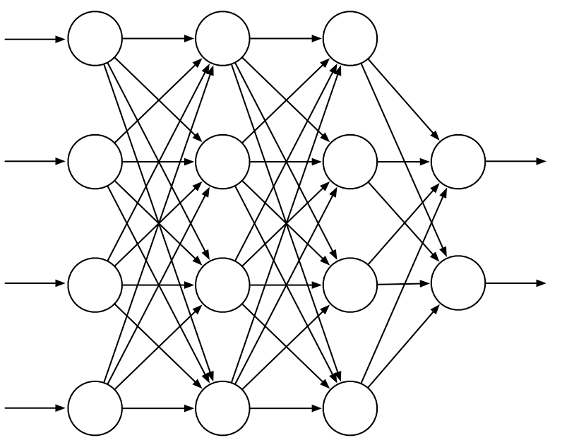
\includegraphics[width=0.4\textwidth]{figures/nn}
    \caption{Generic neural network with two hidden layers}
    \label{fig:nn}
\end{figure}

A generic neural network in \ref{fig:nn} comprises layers of artificial neurons connected with weight, bias vectors, and activation functions to each other. Each activation function feeds nonlinearity to the general equation. 

 

 
